\providecommand{\okm}{{\color{green!55!black}\rule{4pt}{4pt}}~}   %
\providecommand{\badm}{{\color{red!75!black}\rule{4pt}{4pt}}~}    %
\providecommand{\nam}{{\color{black!35}\rule{4pt}{4pt}}~}         %
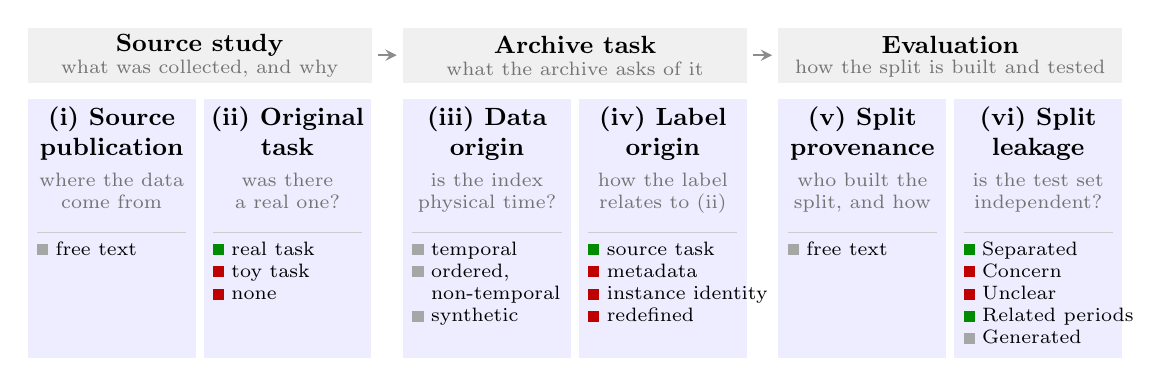
\begin{tikzpicture}[x=1cm,y=1cm,
  >=stealth,
  every node/.style={inner sep=0pt,outer sep=0pt},
  stage/.style  ={fill=black!6},
  field/.style  ={fill=blue!7},
  name/.style   ={font=\small\bfseries, align=center},
  gloss/.style  ={font=\scriptsize, align=center, text=black!55},
  vals/.style   ={font=\scriptsize, align=left},
  arrow/.style  ={->,thick,black!45},
]
\def\W{13.9}    %
\def\SW{4.367}  \def\SG{0.4}    %
\def\FW{2.133}  \def\FG{0.1}    %

\foreach \s/\title/\sgloss in {
  0/Source study/{what was collected, and why},
  1/Archive task/{what the archive asks of it},
  2/Evaluation/{how the split is built and tested}} {
  \pgfmathsetmacro{\x}{\s*(\SW+\SG)}
  \fill[stage] (\x,6.45) rectangle ++(\SW,0.7);
  \node[name]  at (\x+\SW/2,6.93) {\title};
  \node[gloss] at (\x+\SW/2,6.63) {\sgloss};
}
\draw[arrow] (\SW+0.08,6.8) -- ++(\SG-0.16,0);
\draw[arrow] (2*\SW+\SG+0.08,6.8) -- ++(\SG-0.16,0);

\foreach \s/\f/\num/\fname/\fgloss/\fvals in {
  0/0/(i)/{Source\\publication}/{where the data come from}/{\nam free text},
  0/1/(ii)/{Original\\task}/{was there a real one?}/{\okm real task\\ \badm toy task\\ \badm none},
  1/0/(iii)/{Data\\origin}/{is the index physical time?}/{\nam temporal\\ \nam ordered,\\ \phantom{\nam}non-temporal\\ \nam synthetic},
  1/1/(iv)/{Label\\origin}/{how the label relates to (ii)}/{\okm source task\\ \badm metadata\\ \badm instance identity\\ \badm redefined},
  2/0/(v)/{Split\\provenance}/{who built the split, and how}/{\nam free text},
  2/1/(vi)/{Split\\leakage}/{is the test set independent?}/{\okm Separated\\ \badm Concern\\ \badm Unclear\\ \okm Related periods\\ \nam Generated}} {
  \pgfmathsetmacro{\x}{\s*(\SW+\SG)+\f*(\FW+\FG)}
  \fill[field] (\x,2.95) rectangle ++(\FW,3.3);
  \node[name,  anchor=north] at (\x+\FW/2,6.15) {\num~\fname};
  \node[gloss, anchor=north, text width=\FW cm-6pt] at (\x+\FW/2,5.3) {\fgloss};
  \draw[black!20] (\x+0.12,4.55) -- (\x+\FW-0.12,4.55);
  \node[vals,  anchor=north west] at (\x+0.12,4.43) {\fvals};
}

\end{tikzpicture}
